% Provenance (never printed): old terminale S material on the disappearance of
% mountain ranges (erosion, transport, sedimentation, isostatic rebound, the
% recycling of continental material). Owner (Sync 0/1): denudation rate,
% sediment load (bed, suspended, dissolved), isostatic rebound, detrital rock,
% diagenesis. Weathering, erosion, deposition are Book 1's (g5); hydrolysis and
% clay minerals g10.07's; discharge g10.08's; isostasy and Airy's model g11.03's;
% sedimentary basin g11.09's; mountain root g12.01's; metamorphism g12.03's;
% half-life is physics' (recalled in prose). Figures: figdata/grade-12/relief_decay.py
% (rates, decay curves, the Varden unconformity from figdata/shared/region.py).
\chapter{A destruição das montanhas}\label{ch:g12:destruction-of-mountains}

Vistos da Estação Espacial Internacional, os montes Apalaches, no leste da
América do Norte, formam um desenho marcante de longas cristas escuras e
florestadas e de vales claros cultivados, mais de \qty{500}{km} deles na
fotografia abaixo. As cristas são camadas de rocha dura que foram
amarrotadas em \omterm{def:g12:mountain-building:fold}{dobras} apertadas quando a África empurrou a América do Norte,
nos períodos Carbonífero e Permiano, há mais de 250 milhões de anos. Hoje, o
seu cume mais alto, o monte Mitchell, o ponto mais alto a leste do rio
Mississippi, fica a \qty{2037}{m} acima do nível do mar, menos de um quarto
da altura do Everest.
% ledger: photo:g12-appalachians, usgs:alleghanian, usgs:alleghanian-age, ics:base.Triassic, ncparks:mitchell (6684 ft), tht:everest (Book 1 row, 8848.86 m)

\begin{omfigure}
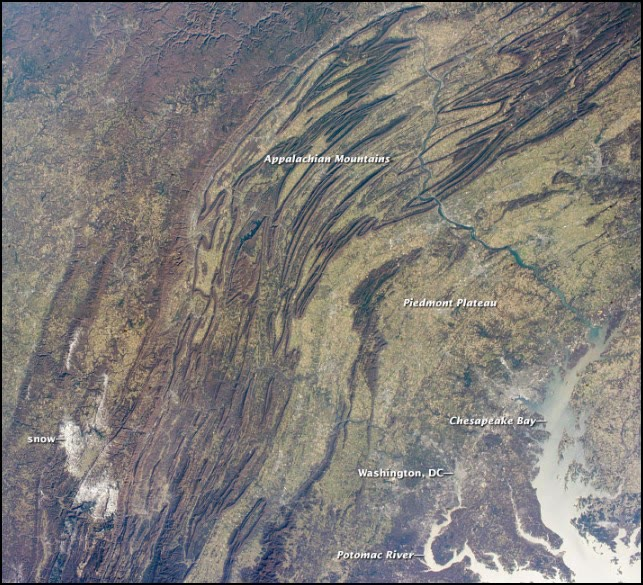
\includegraphics[width=0.6\linewidth]{images/book2/g12-iss-appalachians.jpg}

{\small Os Apalaches de vales e cristas, do nordeste da Pensilvânia (em
cima, à direita) até a Virgínia Ocidental, fotografados da Estação Espacial
Internacional em 17 de novembro de 2012. As cristas florestadas são camadas
de rocha dura, os vales cultivados camadas mais moles. Fotografia NASA
(domínio público).}
\end{omfigure}
% ledger: photo:g12-appalachians

Uma cadeia de montanhas não dura. A partir do momento em que se ergue, a
chuva, o gelo e os rios a atacam; a rocha que eles levam acaba no mar, onde
vira rocha nova. Este capítulo mede a rapidez com que isso acontece,
acompanha os detritos até o lugar onde eles viram pedra, e mostra por que
uma cadeia que está sendo desgastada continua a subir enquanto isso.

\begin{recall}
O intemperismo decompõe a rocha onde ela está; a erosão leva os detritos
embora e a deposição os deposita em outro lugar (Livro 1, 5º ano). O
\omterm{def:g10:soil-formation:chemical-weathering}{intemperismo químico} transforma os feldspatos em \omterm{def:g10:soil-formation:clay}{argilominerais} por
\omterm{def:g10:soil-formation:hydrolysis}{hidrólise} (\cref{ch:g10:soil-formation}). A \omterm{def:g10:drainage-basins:discharge}{vazão} de um rio é o volume de
água que passa por um ponto num segundo (\cref{ch:g10:drainage-basins}). A
crosta flutua sobre o manto em \omterm{def:g11:lithosphere-asthenosphere:isostasy}{isostasia}; no modelo de Airy, uma região cuja
crosta é mais espessa de $\Delta H$ fica mais alta de $\Delta H\,(\rho_m - \rho_c)/\rho_m$
(\cref{ch:g11:lithosphere-asthenosphere}), e uma cadeia alta repousa sobre
uma \omterm{def:g12:continental-crust:root}{raiz} de crosta espessa (\cref{ch:g12:continental-crust}). Os sedimentos
se acumulam em \omterm{def:g11:fossil-fuel-geology:basin}{bacias sedimentares} (\cref{ch:g11:fossil-fuel-geology}). As
rochas enterradas fundo num cinturão de montanhas são metamorfizadas
(\cref{ch:g12:metamorphic-rocks}).
\end{recall}

\section{A que velocidade a terra é desgastada?}

\begin{definition}[Taxa de denudação]\label{def:g12:destruction-of-mountains:denudation}
A \emph{taxa de denudação}\index{taxa de denudacao@taxa de denudação} de uma região é a
espessura média de rocha que o intemperismo e a erosão juntos removem dela
por unidade de tempo. Ela é dada em geral em metros por milhão de anos
(\unit{m/Myr}), o que é o mesmo que milímetros por mil anos.
\end{definition}
% ledger: pb11:rates (rates in m/Myr), earle:loads

Como medir algo tão lento? Os raios cósmicos que atingem o solo produzem um
isótopo raro, o berílio-10, no quartzo dos primeiros metros de rocha. Quanto
mais lentamente uma superfície é desgastada, mais tempo cada grão fica perto
do topo, e mais berílio-10 ele acumula. Medi-lo na areia de um rio dá a \omterm{def:g12:destruction-of-mountains:denudation}{taxa
média de denudação} de toda a bacia a montante, ao longo dos últimos milhares
a milhões de anos.
% ledger: pb11:rates (10Be produced within a few metres of the surface; concentration reflects near-surface residence time; 10^3 to 10^6 years)

Uma compilação de 1599 medições desse tipo constatou que os afloramentos de
rocha nua são desgastados lentamente, em \qty{12}{m/Myr} em média (mediana
de \qty{5.4}{m/Myr}), e nunca mais depressa que \qty{140}{m/Myr}. As \omterm{def:g10:drainage-basins:drainage-basin}{bacias
hidrográficas} inteiras perdem muito mais, \qty{218}{m/Myr} em média, mas com
uma mediana de só \qty{54}{m/Myr}: algumas bacias rápidas puxam a média para
cima. As mais rápidas são as íngremes: a declividade média de uma bacia é o
fator que melhor prevê a sua taxa. As bacias de regiões sismicamente ativas,
onde as montanhas estão subindo, são erodidas cerca de duas vezes mais
depressa que as de regiões tranquilas.
% ledger: pb11:rates

\begin{omfigure}
\begin{tikzpicture}
\begin{axis}[omrecord, xbar, xmode=log, log origin=infty, bar width=7pt, bar shift=0pt,
  width=0.62\linewidth, height=6.6cm, scale only axis, xmin=3, xmax=1000,
  ymin=0.4, ymax=10.6, ytick={1,...,10}, y tick label style={font=\scriptsize, align=right},
  yticklabels={{afloramentos, mediana}, {afloramentos, média}, {rios do mundo (balanço)}, {bacias, mediana},
    {Mississippi, antes de 1900 (balanço)}, {bacias áridas, média}, {bacias tranquilas, média}, {bacias, média},
    {bacias sismicamente ativas, média}, {bacias polares, média}},
  xlabel={taxa de denudação (\unit{m/Myr}), escala logarítmica}, ymajorgrids=false,
  unbounded coords=discard, nodes near coords, nodes near coords align={horizontal}, nodes near coords style={font=\scriptsize},
  point meta=rawx, every node near coord/.append style={/pgf/number format/.cd, fixed, precision=0}]
% computed in figdata/grade-12/relief_decay.py; ledger: pb11:rates, mm10:mississippi, kammerer:mississippi, earle:loads, cm95:crust
\addplot[fill=omThm!45, draw=omThm, every node near coord/.append style={/pgf/number format/.cd, fixed, precision=1}] table[x=measured, y=idx] {figdata/out/grade-12-relief_decay-rates.dat};
\addplot[fill=omDef!45, draw=omDef] table[x=budget, y=idx] {figdata/out/grade-12-relief_decay-rates.dat};
\end{axis}
\end{tikzpicture}

{\small \omterm{def:g12:destruction-of-mountains:denudation}{Taxas de denudação} medidas com o berílio-10 (em vermelho: 1599
medições, 1149 delas em areia de rio) e duas taxas calculadas neste capítulo
a partir do sedimento que os rios carregam (em azul). Fontes: Portenga e
Bierman (2011); Meade e Moody (2010); Syvitski e colaboradores (2005).}
\end{omfigure}
% values: world_m_per_myr 43.5, miss_before_1900_m_per_myr 55.8 (relief_decay.py)

\section{Os rios levam as montanhas embora}

Grande parte do que é desgastado da terra a deixa nos rios.

\begin{definition}[Carga sedimentar]\label{def:g12:destruction-of-mountains:load}
A \emph{carga sedimentar}\index{carga sedimentar} de um rio é o material que
ele carrega, sob três formas: a \emph{carga de fundo}\index{carga de fundo},
grãos grandes rolados, empurrados ou saltitando ao longo do leito; a
\emph{carga em suspensão}\index{carga em suspensao@carga em suspensão},
grãos pequenos mantidos na água em movimento; e a \emph{carga
dissolvida}\index{carga dissolvida}, íons em solução, como o cálcio e o
cloreto, deixados pelo \omterm{def:g10:soil-formation:chemical-weathering}{intemperismo químico}.
\end{definition}
% ledger: earle:loads

Em média, a \omterm{def:g12:destruction-of-mountains:load}{carga dissolvida} é cerca de \qty{15}{\percent} da massa que um
rio carrega. Quanto mais rápida a água, maiores os grãos que ela pode
levantar. Um grão de areia de \qty{1}{mm} de diâmetro é retirado do leito a
cerca de \qty{20}{cm/s}, e uma vez em movimento continua em suspensão até
que a corrente caia abaixo de \qty{10}{cm/s}. Os grãos de silte são mais
difíceis de levantar que a areia, porque grudam uns nos outros: um grão de
\qty{0.01}{mm} precisa de \qty{60}{cm/s} para ser levantado, mas depois uma
corrente de \qty{0.1}{cm/s} o mantém em suspensão. É por isso que os rios em
cheia correm marrons, e que a lama mais fina viaja até o mar.
% ledger: earle:loads

\begin{omfigure}
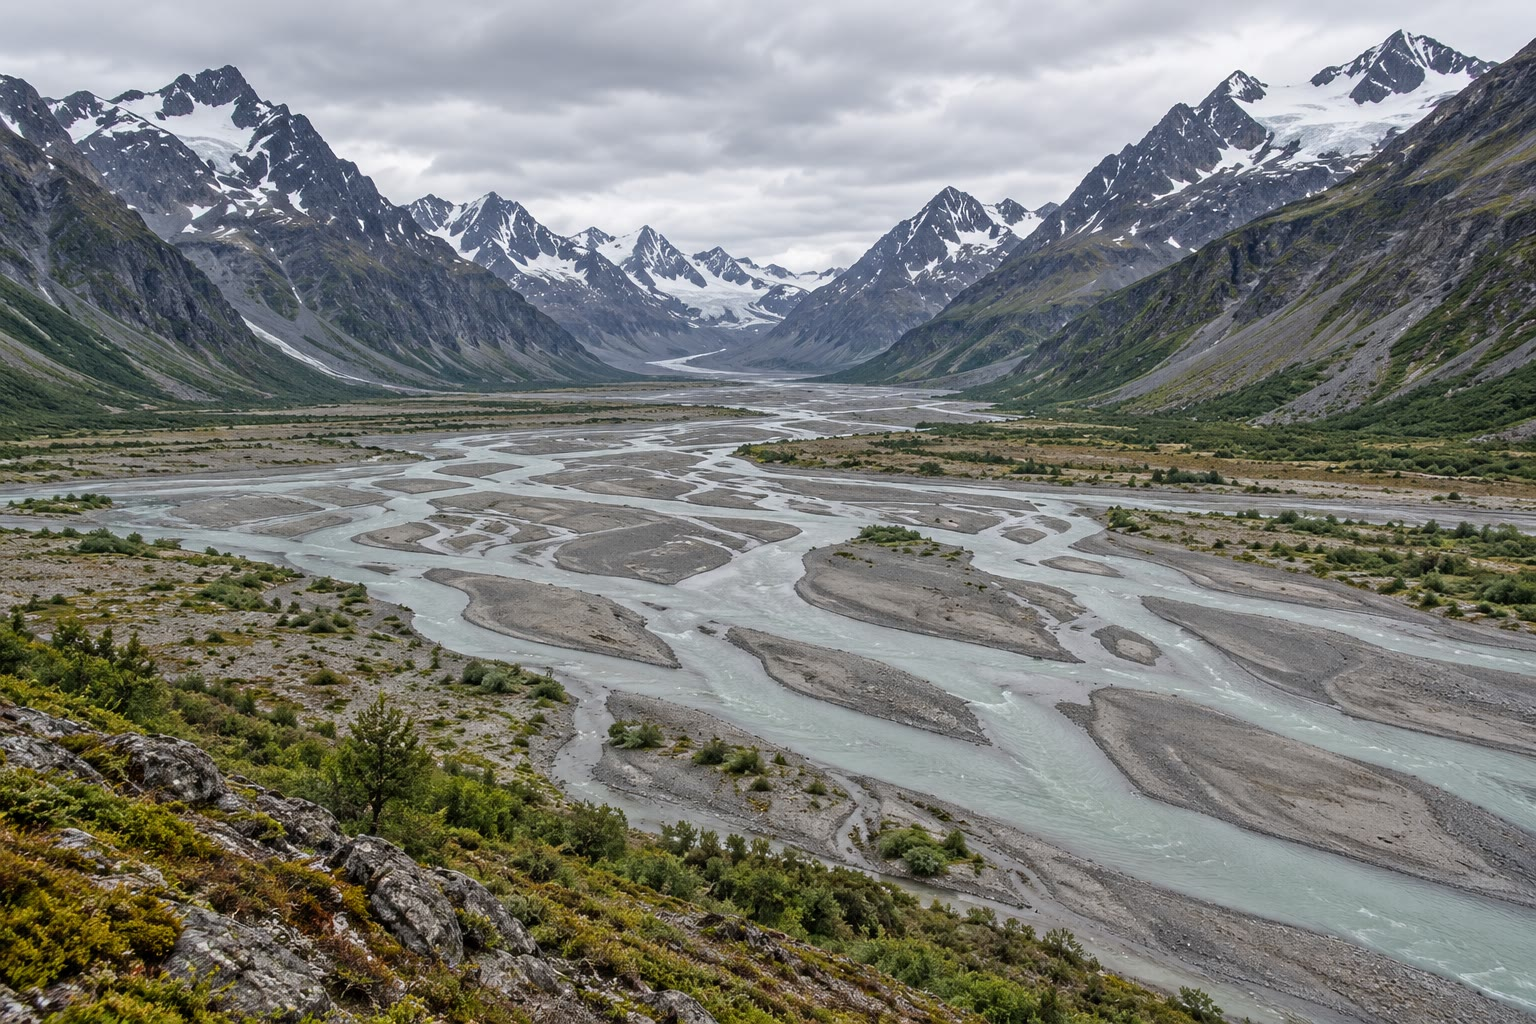
\includegraphics[width=0.66\linewidth]{images/book2/ai/g12-braided-river.jpg}

{\small Um rio entrelaçado num vale glacial de montanha: canais rasos se
dividem e se juntam de novo entre barras de cascalho que a água só move nas
cheias. Ilustração gerada por IA.}
\end{omfigure}

Medir o que um rio carrega dá uma segunda maneira de encontrar uma \omterm{def:g12:destruction-of-mountains:denudation}{taxa de
denudação}.

\begin{method}[Um balanço de erosão]\label{met:g12:destruction-of-mountains:budget}
\begin{enumerate}
  \item Tome a massa de sedimento que o rio carrega em um ano, e some a
        \omterm{def:g12:destruction-of-mountains:load}{carga dissolvida} (se só a carga sólida é conhecida, divida-a por
        $0.85$).
  \item Divida pela densidade da rocha, cerca de \qty{2830}{kg/m^3} para a
        \omterm{def:g12:continental-crust:continental-crust}{crosta continental}, para obter o volume de rocha removido a cada
        ano.
  \item Divida pela área da \omterm{def:g10:drainage-basins:drainage-basin}{bacia hidrográfica}: é a espessura removida a
        cada ano.
  \item Multiplique por $10^6$ para expressá-la em metros por milhão de
        anos.
\end{enumerate}
\end{method}
% ledger: earle:loads, cm95:crust

\begin{example}[O Mississippi]\label{ex:g12:destruction-of-mountains:mississippi}
Antes de 1900, o sistema fluvial Missouri--Mississippi levava cerca de 400
milhões de toneladas de sedimento por ano ao mar, de uma bacia de cerca de
\qty{2980000}{km^2}. Com a \omterm{def:g12:destruction-of-mountains:load}{carga dissolvida}, $400/0.85 \approx 471$ milhões
de toneladas, isto é, $\num{4.71e11}/2830 \approx \qty{1.66e8}{m^3}$ de
rocha por ano. Espalhados sobre $\qty{2.98e12}{m^2}$, eles formam uma camada
\[
  \frac{\num{1.66e8}}{\num{2.98e12}} \approx \qty{5.6e-5}{m}
  \text{ por ano, cerca de } \qty{56}{m/Myr}.
\]
Entre 1987 e 2006, o rio levou só 145 milhões de toneladas por ano, o que
dá cerca de \qty{20}{m/Myr}: as barragens construídas no Missouri nos anos
1950 retêm cerca de 100 a 150 milhões de toneladas por ano, e outras obras
retêm mais.
\end{example}
% ledger: mm10:mississippi, kammerer:mississippi, earle:loads, cm95:crust
% values: miss_before_1900_m_per_myr 55.8, miss_1987_2006_m_per_myr 20.2 (relief_decay.py)

O mesmo balanço pode ser feito para o mundo inteiro. Antes que as pessoas
mudassem os rios, eles levavam cerca de 15.5 bilhões de toneladas de
sedimento sólido por ano às costas; com a \omterm{def:g12:destruction-of-mountains:load}{carga dissolvida}, são cerca de
\qty{6.4}{km^3} de rocha por ano, tirados dos \qty{1.48e8}{km^2} dos
continentes: uma \omterm{def:g12:destruction-of-mountains:denudation}{taxa média de denudação} de cerca de \qty{43}{m/Myr}, perto
da mediana das medições de berílio-10. Desde então, as pessoas mudaram os
dois termos: a erosão dos solos aumentou o que os rios recolhem em cerca de
2.3 bilhões de toneladas por ano, mas mais de 100 bilhões de toneladas de
sedimento estão hoje retidas atrás de barragens.
% ledger: syvitski:modern-flux (Book 1 row, prehuman 15.5 Gt/yr with bed load), sy05:humans, data:etopo1 (land fraction 0.290, grade-11 hypsometry), cm95:crust
% values: world_volume_km3_per_yr 6.44, land_area_km2 1.48e8, world_m_per_myr 43.5 (relief_decay.py)

\section{Do sedimento à rocha}

O que os rios carregam é depositado onde a corrente diminui: nos vales e nos
lagos, nos deltas, e sobretudo nas \omterm{def:g11:fossil-fuel-geology:basin}{bacias sedimentares} das margens
continentais. Camada após camada, o sedimento é enterrado, e lentamente se
transforma em rocha.

\begin{definition}[Rocha detrítica; diagênese]\label{def:g12:destruction-of-mountains:diagenesis}
Uma \emph{rocha detrítica}\index{rocha detritica@rocha detrítica} (ou rocha clástica) é uma
rocha sedimentar feita de fragmentos, os clastos, de rochas e minerais mais
antigos. A \emph{diagênese}\index{diagenese@diagênese} é o conjunto das
mudanças que transformam um sedimento enterrado em rocha a baixa
temperatura: a \emph{compactação}, quando o peso das camadas de cima expulsa
a água e o ar, e depois a \emph{cimentação}, quando minerais que se
cristalizam a partir da água dos poros (calcita, quartzo, hematita,
\omterm{def:g10:soil-formation:clay}{argilominerais}) colam os grãos uns aos outros.
\end{definition}
% ledger: earle:clastic

As \omterm{def:g12:destruction-of-mountains:diagenesis}{rochas detríticas} são nomeadas pelo tamanho dos seus clastos:
\begin{itemize}
  \item um \textbf{conglomerado} é feito de clastos arredondados maiores que
        \qty{2}{mm}, uma \textbf{brecha} de clastos angulosos;
  \item um \textbf{arenito} é feito de areia, grãos entre \qty{2}{mm}
        e \qty{0.063}{mm}, na maioria das vezes de quartzo, o mineral que
        melhor resiste ao intemperismo;
  \item um \textbf{lamito} contém pelo menos \qty{75}{\percent} de silte e
        de argila; é um folhelho se ele se parte em camadas finas.
\end{itemize}
% ledger: earle:clastic

\begin{omfigure}
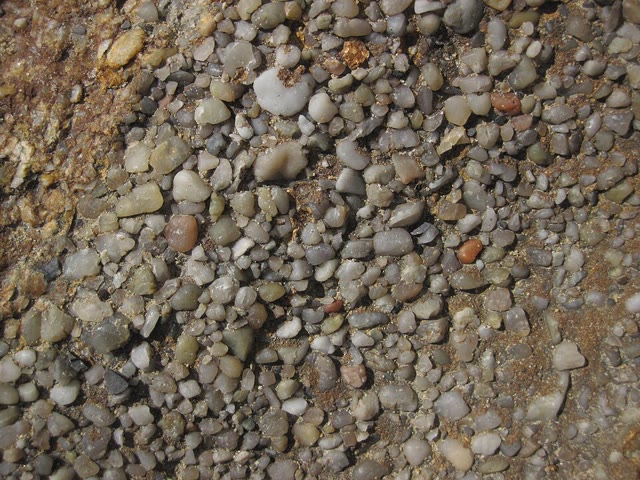
\includegraphics[width=0.5\linewidth]{images/book2/g12-stjohn-conglomerate.jpg}

{\small Um conglomerado de seixos de quartzo de Ohio, da idade carbonífera:
seixos arredondados de quartzo, cimentados por uma areia mais fina.
Fotografia James St.~John (CC~BY~2.0).}
\end{omfigure}
% ledger: photo:g12-conglomerate, ics:base.Carboniferous, ics:base.Permian (Lower Pennsylvanian lies in the Carboniferous)

Os clastos registram a viagem. Os seixos arredondados rolaram muito num rio
ou numa praia; os angulosos quase não viajaram. Um arenito feito quase só
de quartzo vem de uma rocha que foi intemperizada por muito tempo, até que
os outros minerais tivessem virado argila.
% ledger: earle:clastic (rounded/angular, most sand grains quartz, the most resistant mineral)

\section{A raiz sobe}

Se a erosão simplesmente removesse rocha do topo de uma cadeia, uma cadeia
de \qty{2}{km} de altura, desgastada a \qty{200}{m/Myr}, desapareceria em
dez milhões de anos. Mas a cadeia flutua sobre o manto. À medida que a rocha
é removida do topo, a coluna fica mais leve, e sobe.

\begin{definition}[Rebote isostático]\label{def:g12:destruction-of-mountains:rebound}
O \emph{rebote isostático}\index{rebote isostatico@rebote isostático} é a subida de uma região
da \omterm{def:g11:lithosphere-asthenosphere:lithosphere}{litosfera} quando uma carga é removida dela --- rocha desgastada pela
erosão, ou uma calota de gelo que derrete --- até que a \omterm{def:g11:lithosphere-asthenosphere:isostasy}{isostasia} seja
restabelecida.
\end{definition}
% ledger: sella07:gia (rebound after ice unloading)

\begin{proposition}[Erosão e rebote]\label{prop:g12:destruction-of-mountains:rebound}
No modelo de Airy, quando a erosão remove uma espessura $e$ de crosta de
densidade $\rho_c$ de uma região em \omterm{def:g11:lithosphere-asthenosphere:isostasy}{isostasia} sobre um manto de densidade
$\rho_m$, a superfície desce apenas
\[
  \Delta h = e\left(1 - \frac{\rho_c}{\rho_m}\right),
\]
enquanto a base da crosta sobe $e\,\rho_c/\rho_m$.
\end{proposition}

\begin{proof}
Remover $e$ do topo torna a crosta mais fina de $e$. Pelo modelo de Airy,
uma crosta mais fina de $e$ fica mais baixa de $e\,(\rho_m - \rho_c)/\rho_m = e(1 -
\rho_c/\rho_m)$. O topo da crosta desceu dessa quantidade, e a sua espessura
diminuiu de $e$, logo a sua base subiu $e - e(1 -
\rho_c/\rho_m) = e\,\rho_c/\rho_m$.
\end{proof}

Com $\rho_c = \qty{2830}{kg/m^3}$ e $\rho_m = \qty{3380}{kg/m^3}$, $1 -
\rho_c/\rho_m \approx 0.163$. Remover \qty{1}{km} de rocha abaixa a
superfície em apenas cerca de \qty{163}{m}: os outros \qty{837}{m} são
compensados pela subida de toda a coluna. Para abaixar uma cadeia em
\qty{2000}{m}, a erosão precisa remover cerca de
$2000/0.163 \approx \qty{12300}{m}$ de rocha. Rochas que estavam a mais de
\qty{12}{km} de profundidade, rochas metamórficas e granitos formados nas
profundezas da cadeia, chegam à superfície: é por isso que os antigos
cinturões de montanhas desgastados expõem xistos, gnaisses e granitos em
vastas áreas.
% ledger: cm95:crust, data:prem (rho 3.38 below the Moho)
% values: rebound_fraction 0.16272, lowering_per_km_m 162.7, root_rise_per_km_m 837.3, eroded_for_2000m_km 12.29 (relief_decay.py)

\begin{omfigure}
\begin{tikzpicture}[x=1cm, y=1cm, font=\scriptsize]
  % three columns: before, after erosion without rebound, after rebound
  \foreach \i/\top/\base/\lab in {0/3.0/-3.2/{uma cadeia em isostasia}, 1/2.0/-3.2/{a erosão remove $e$}, 2/2.84/-2.36/{a coluna sobe}} {
    \begin{scope}[xshift=\i*4.6cm]
      \fill[omLithPeridotite!45] (0,-3.6) rectangle (3.4,-0.6);
      \fill[omLithGranite!55, draw=black!60] (0.5,\base) -- (0.5,0) -- (1.0,\top) -- (2.4,\top) -- (2.9,0) -- (2.9,\base) -- cycle;
      \fill[omLithGranite!55, draw=black!60] (0,0) rectangle (0.5,-0.6);
      \fill[omLithGranite!55, draw=black!60] (2.9,0) rectangle (3.4,-0.6);
      \draw[black!40, densely dashed] (-0.1,0) -- (3.5,0);
      \node[anchor=north, align=center, text width=3.4cm] at (1.7,-3.75) {\lab};
    \end{scope}
  }
  % eroded slab, middle panel
  \draw[omThm, densely dashed] (4.6+1.0,3.0) -- (4.6+2.4,3.0);
  \draw[omThm, |-|] (4.6+2.65,3.0) -- node[right] {$e$} (4.6+2.65,2.0);
  % right panel: the old top and base
  \draw[omThm, densely dashed] (9.2+1.0,3.0) -- (9.2+2.4,3.0);
  \draw[omThm, densely dashed] (9.2+0.5,-3.2) -- (9.2+2.9,-3.2);
  \draw[-{Stealth}, omDef, line width=0.9pt] (9.2+1.7,-3.15) -- (9.2+1.7,-2.45);
  \node[omDef, anchor=west] at (9.2+3.0,-2.8) {a raiz sobe};
  \node[anchor=west] at (9.2+3.0,2.95) {superfície mais baixa};
  \node[anchor=west] at (9.2+3.0,2.55) {só de $0.16\,e$};
  \draw[black!60, |-|] (9.2+2.65,3.0) -- (9.2+2.65,2.84);
  % labels
  \node[anchor=west] at (3.45,-2.1) {manto};
  \node at (1.7,-1.5) {crosta};
\end{tikzpicture}

{\small Erosão e \omterm{def:g12:destruction-of-mountains:rebound}{rebote isostático} (esquemático, alturas fora de escala). À
esquerda: uma cadeia em \omterm{def:g11:lithosphere-asthenosphere:isostasy}{isostasia}, com a sua \omterm{def:g12:continental-crust:root}{raiz}. No meio: a erosão remove
uma espessura $e$ do topo. À direita: a coluna mais leve sobe até que a
\omterm{def:g11:lithosphere-asthenosphere:isostasy}{isostasia} seja restabelecida; a superfície termina apenas $0.163\,e$ mais
baixa que no início, e a \omterm{def:g12:continental-crust:root}{raiz} subiu $0.837\,e$.}
\end{omfigure}

O mesmo rebote pode ser observado hoje onde uma carga desapareceu depressa.
A calota de gelo que cobria grande parte do Canadá no último máximo glacial
era mais espessa em volta da baía de Hudson. Esse gelo derreteu, e a terra
ali ainda está subindo: cerca de \qty{10}{mm} por ano, medidos por GPS, isto
é, \qty{10000}{m/Myr}, cerca de cinquenta vezes a \omterm{def:g12:destruction-of-mountains:denudation}{taxa média de denudação}
das \omterm{def:g10:drainage-basins:drainage-basin}{bacias hidrográficas}. Mais ao sul,
além dos Grandes Lagos, a terra afunda de 1 a \qty{2}{mm} por ano.
% ledger: sella07:gia, pb11:rates

\section{Quanto tempo dura uma cadeia?}

Quanto mais íngreme uma bacia, mais depressa ela é erodida; para as grandes
bacias, constatou-se que a \omterm{def:g12:destruction-of-mountains:denudation}{taxa de denudação} é proporcional ao seu relevo
médio. Tomemos o modelo mais simples que diz isso.

\begin{proposition}[O decaimento exponencial de uma cadeia]\label{prop:g12:destruction-of-mountains:decay}
Seja $h(t)$ a altitude média de uma cadeia acima das planícies em volta. Se
a \omterm{def:g12:destruction-of-mountains:denudation}{taxa de denudação} é $E = k\,h$, com $k$ uma constante, e se a \omterm{def:g11:lithosphere-asthenosphere:isostasy}{isostasia} é
restabelecida o tempo todo, então
\[
  h(t) = h_0\, e^{-f k t}, \qquad f = 1 - \frac{\rho_c}{\rho_m},
\]
em que $h_0$ é a altitude em $t = 0$. A altitude é dividida por $e$
a cada $\tau = 1/(fk)$, e por dois a cada $\tau \ln 2$.
\end{proposition}

\begin{proof}
Num tempo curto $\mathrm{d}t$, a erosão remove uma espessura $E\,\mathrm{d}t
= k h\,\mathrm{d}t$, e pela proposição anterior a superfície desce
$f k h\,\mathrm{d}t$. Logo $h' = -fk\,h$, e as soluções dessa
equação são $h(t) = h_0\,e^{-fkt}$. Em $t = \tau$, $h = h_0/e$; $h = h_0/2$
quando $fkt = \ln 2$.
\end{proof}

As medições em grandes bacias dão $k$: sem nenhum soerguimento, o seu relevo
cairia a um décimo em cerca de 11 milhões de anos. Logo $e^{-11k} = 0.1$, e
$k =
\ln 10/11 \approx 0.209$ por milhão de anos. Sem rebote ($f = 1$), a
constante de tempo seria $1/k \approx 4.8$ milhões de anos. Com rebote, $f
\approx 0.163$ e
\[
  \tau = \frac{1}{0.163 \times 0.209} \approx 29 \text{ milhões de anos},
\]
e a altitude média se reduz à metade a cada $29 \ln 2 \approx 20$ milhões
de anos: o rebote faz uma cadeia durar cerca de seis vezes mais.
% ledger: ahnert70:decay, cm95:crust, data:prem
% values: k_per_myr 0.20933, tau_none_myr 4.777, tau_rebound_myr 29.36, half_rebound_myr 20.35, half_none_myr 3.31 (relief_decay.py)

\begin{omfigure}
\begin{tikzpicture}
\begin{axis}[omrecord, width=0.7\linewidth, height=5.4cm, xmin=0, xmax=100, ymin=0, ymax=2100,
  xlabel={tempo (milhões de anos)}, ylabel={altitude média (\unit{m})},
  xtick={0,20,...,100}, ytick={0,500,...,2000}]
% computed in figdata/grade-12/relief_decay.py; ledger: ahnert70:decay, cm95:crust, data:prem
\addplot[omProp, line width=1.1pt, densely dashed] table[x=t_Myr, y=h_none] {figdata/out/grade-12-relief_decay-curve.dat};
\addplot[omDef, line width=1.1pt] table[x=t_Myr, y=h_rebound] {figdata/out/grade-12-relief_decay-curve.dat};
\draw[black!45, densely dotted] (axis cs:20.35,0) -- (axis cs:20.35,1000) -- (axis cs:0,1000);
\draw[omProp, line width=0.4pt] (axis cs:9,304) -- (axis cs:33,215);
\coordinate (none) at (axis cs:33.5,215);
\coordinate (reb) at (axis cs:45,780);
\end{axis}
\node[font=\scriptsize, text=omProp, anchor=west] at (none) {sem rebote};
\node[font=\scriptsize, text=omDef, anchor=south west] at (reb) {com rebote};
\end{tikzpicture}

{\small A altitude média de uma cadeia de \qty{2000}{m} de altura,
desgastada a uma taxa proporcional à sua altura, com e sem \omterm{def:g12:destruction-of-mountains:rebound}{rebote
isostático}; com rebote, resta a metade da altitude depois de 20 milhões de
anos (pontilhado). Constante de taxa segundo Ahnert (1970); densidades da
crosta e do manto abaixo do \omterm{def:g11:seismic-structure:moho}{Moho}.}
\end{omfigure}

Os Apalaches põem esse quadro à prova. A sua colisão terminou no Permiano,
há mais de 250 milhões de anos. É mais de doze vezes o tempo que o modelo
leva para reduzir a altitude à metade: $2000 \times e^{-250/29} \approx
\qty{0.4}{m}$. No entanto, o monte Mitchell ainda se ergue a \qty{2037}{m}
acima do mar. O modelo sozinho não pode explicar o relevo atual: a região
deve ter sido erguida de novo desde então, ou erodida mais lentamente do
que o modelo supõe.
% ledger: usgs:alleghanian, usgs:alleghanian-age, ics:base.Triassic, ncparks:mitchell, ahnert70:decay
% values: h_after_250myr_rebound_m 0.40 (relief_decay.py)

Assim, as montanhas são recicladas. A rocha desgastada de uma cadeia acaba
em \omterm{def:g11:fossil-fuel-geology:basin}{bacias sedimentares}, onde vira \omterm{def:g12:destruction-of-mountains:diagenesis}{rocha detrítica}; uma parte dessa rocha é
enterrada fundo o bastante para ser metamorfizada ou até para se fundir,
uma parte é levada para o manto numa \omterm{def:g11:subduction-zones:subduction}{zona de subducção}
(\cref{ch:g12:subduction-magmatism}), e uma parte é dobrada de novo numa
nova cadeia quando dois continentes colidem.
% ledger: ss09:balance (sediment subducted), earle:collision (sediments of both margins in the mountains)

\begin{omfigure}
\begin{tikzpicture}
\begin{axis}[omsection, x=1.25cm, y=0.003125cm, xmin=0, xmax=9.49, ymin=-700, ymax=650,
  xlabel={distância a partir de A (\unit{km})}, ylabel={altitude (\unit{m})},
  ytick={-600,-300,0,300,600}, tick label style={font=\scriptsize}, unbounded coords=jump]
% shared region tables (figdata/shared/region.py); unconformity from figdata/grade-12/relief_decay.py; ledger: region:name
\addplot[fill=black!8, draw=black!50, line width=0.3pt, even odd rule] table {figdata/out/shared-region-section-unit-schist.dat};
\addplot[fill=icsTriassic!20, draw=black!50, line width=0.3pt, even odd rule] table {figdata/out/shared-region-section-unit-sandstone.dat};
\addplot[fill=icsJurassic!25, draw=black!50, line width=0.3pt, even odd rule] table {figdata/out/shared-region-section-unit-limestone.dat};
\addplot[fill=icsJurassic!8, draw=black!50, line width=0.3pt, even odd rule] table {figdata/out/shared-region-section-unit-shale.dat};
\addplot[fill=icsCretaceous!20, draw=black!50, line width=0.3pt, even odd rule] table {figdata/out/shared-region-section-unit-chalk.dat};
\addplot[fill=omLithAlluv, draw=black!50, line width=0.3pt, even odd rule] table {figdata/out/shared-region-section-unit-alluvium.dat};
\addplot[black, line width=0.7pt] table {figdata/out/shared-region-section-ground.dat};
\addplot[omThm, line width=1.4pt] table[x=s_km, y=z_m] {figdata/out/grade-12-relief_decay-unconformity.dat};
\addplot[fault] table {figdata/out/shared-region-section-fault.dat};
\node[anchor=south east, font=\small\bfseries] at (axis cs:0,650) {A};
\node[anchor=south west, font=\small\bfseries] at (axis cs:9.49,650) {B};
\node[font=\scriptsize, fill=white, inner sep=1pt] at (axis cs:1.2,-520) {xisto, cerca de 480 Ma};
\coordinate (unc) at (axis cs:1.6,-300);
\end{axis}
\node[font=\scriptsize, text=omThm, anchor=west, fill=white, inner sep=1pt] at ([xshift=4pt]unc) {a discordância};
\end{tikzpicture}

\smallskip
{\small\tikz\fill[black!8, draw=black!50] (0,0) rectangle (0.35,0.22);~xisto \quad
\tikz\fill[icsTriassic!20, draw=black!50] (0,0) rectangle (0.35,0.22);~arenito (Triássico) \quad
\tikz\fill[icsJurassic!25, draw=black!50] (0,0) rectangle (0.35,0.22);~calcário \quad
\tikz\fill[icsJurassic!8, draw=black!50] (0,0) rectangle (0.35,0.22);~folhelho \quad
\tikz\fill[icsCretaceous!20, draw=black!50] (0,0) rectangle (0.35,0.22);~giz \quad
\omve{2.5}}

{\small Corte A--B através das Colinas de Varden, com a discordância em
vermelho: a base plana sobre a qual o arenito triássico foi depositado por
cima do embasamento de xisto, mais tarde dobrada e falhada. Dados: o modelo
da região usado nesta série.}
\end{omfigure}
% values: unconformity sampled from region.contact_elevation('sandstone'); varden_gap_myr 58.1 (relief_decay.py)

As Colinas de Varden guardam o registro de um ciclo assim. O seu
embasamento é um xisto, metamorfizado há cerca de 480 milhões de anos, no
qual um granito se intrudiu há cerca de 310 milhões de anos --- ambos
formados a quilômetros abaixo da superfície de um antigo cinturão de
montanhas. No entanto, o arenito triássico, depositado a partir de cerca de
252 milhões de anos atrás, repousa diretamente sobre eles, através de uma
superfície plana: a discordância. Em menos de 60 milhões de anos, aquela
antiga cadeia tinha sido desgastada até virar uma planície e as suas rochas
profundas trazidas à superfície. O mar então se espalhou sobre a planície e
a soterrou.
% ledger: region:name (model: schist 480 Ma, granite 310 Ma, erosion, unconformity, Triassic cover), ics:base.Triassic
% values: varden_gap_myr 58.1 (relief_decay.py)

\section{Exercícios}

\begin{exercise}[$\star$]\label{exo:g12:destruction-of-mountains:1}
Dê a palavra: (a) a espessura média de rocha removida de uma região por
unidade de tempo; (b) os grãos que um rio rola e faz saltar ao longo do seu
leito; (c) os íons que um rio carrega em solução; (d) as mudanças que
transformam um sedimento enterrado em rocha; (e) a subida da \omterm{def:g11:lithosphere-asthenosphere:lithosphere}{litosfera}
quando uma carga é removida dela.
\end{exercise}

\begin{exercise}[$\star$]\label{exo:g12:destruction-of-mountains:2}
Dê o nome da \omterm{def:g12:destruction-of-mountains:diagenesis}{rocha detrítica}: (1) seixos arredondados de \qtyrange{5}{20}{mm}
cimentados entre si; (2) grãos de quartzo de \qty{0.3}{mm}; (3) uma rocha
com \qty{90}{\percent} de silte e de argila que se parte em placas finas;
(4) fragmentos angulosos de \qty{3}{cm}.
\end{exercise}

\begin{exercise}[$\star$]\label{exo:g12:destruction-of-mountains:3}
Converta em milímetros por ano: (1) \qty{54}{m/Myr}; (2) \qty{218}{m/Myr};
(3) a subida de \qty{10}{mm} por ano perto da baía de Hudson, em \unit{m/Myr}.
\end{exercise}

\begin{exercise}[$\star$]\label{exo:g12:destruction-of-mountains:4}
Um rio carrega 60 milhões de toneladas de sedimento sólido por ano. Estime
a sua \omterm{def:g12:destruction-of-mountains:load}{carga dissolvida}, sabendo que a \omterm{def:g12:destruction-of-mountains:load}{carga dissolvida} é em média
\qty{15}{\percent} da massa total carregada.
\end{exercise}

\begin{exercise}[$\star$]\label{exo:g12:destruction-of-mountains:5}
Ponha em ordem, da superfície para baixo, o que acontece com um grão de
quartzo de um granito: deposição numa bacia, intemperismo do granito,
soterramento sob camadas mais jovens, transporte por um rio, cimentação.
\end{exercise}

\begin{exercise}[$\star\star$]\label{exo:g12:destruction-of-mountains:6}
Uma corrente diminui de \qty{30}{cm/s} para \qty{5}{cm/s}. Usando os valores
do capítulo, diga o que acontece com um grão de areia de \qty{1}{mm} pousado
no leito, e com um grão de silte de \qty{0.01}{mm} já em suspensão, a cada
velocidade.
\end{exercise}

\begin{exercise}[$\star\star$]\label{exo:g12:destruction-of-mountains:7}
Uma bacia de \qty{50000}{km^2} envia 4 milhões de toneladas de sedimento
sólido por ano ao mar. Faça o seu balanço de erosão, \omterm{def:g12:destruction-of-mountains:load}{carga dissolvida}
incluída, com $\rho =
\qty{2830}{kg/m^3}$. Compare com a mediana das taxas de berílio-10 das
bacias.
\end{exercise}

\begin{exercise}[$\star\star$]\label{exo:g12:destruction-of-mountains:8}
(1) Calcule $1 - \rho_c/\rho_m$ para $\rho_c = \qty{2700}{kg/m^3}$ e
$\rho_m = \qty{3300}{kg/m^3}$. (2) Quanto a superfície abaixa quando
\qty{1}{km} de rocha é erodido? (3) Compare com o valor do capítulo.
\end{exercise}

\begin{exercise}[$\star\star$]\label{exo:g12:destruction-of-mountains:9}
Um granito se cristalizou a cerca de \qty{8}{km} de profundidade sob uma
cadeia. (1) Que espessura de rocha a erosão precisa remover para trazê-lo à
superfície? (2) Quanto a superfície média desce enquanto isso? (3) A
\qty{200}{m/Myr}, quanto tempo isso leva?
\end{exercise}

\begin{exercise}[$\star\star$]\label{exo:g12:destruction-of-mountains:10}
A altitude média dos continentes é de cerca de \qty{794}{m}. (1) A
\qty{43}{m/Myr}, quanto tempo a erosão levaria para remover uma camada dessa
espessura? (2) Quanto tempo, se o \omterm{def:g12:destruction-of-mountains:rebound}{rebote isostático} for levado em conta e a
taxa continuar a mesma? (3) Por que os continentes, ainda assim, continuam
acima do mar depois de 4 bilhões de anos?
\end{exercise}

\begin{exercise}[$\star\star$]\label{exo:g12:destruction-of-mountains:11}
Mais de 100 bilhões de toneladas de sedimento estão retidas atrás de
barragens construídas em sua maioria nos últimos cinquenta anos. (1) Que
volume de rocha é esse, a
\qty{2830}{kg/m^3}? (2) Quantos anos da carga sólida pré-humana do mundo,
15.5 bilhões de toneladas por ano, ele representa?
\end{exercise}

\begin{exercise}[$\star\star\star$]\label{exo:g12:destruction-of-mountains:12}
Mostre que, no modelo do capítulo, a \omterm{def:g12:destruction-of-mountains:denudation}{taxa de denudação} de uma cadeia é
$E(t) = k h_0 e^{-fkt}$. Calcule a espessura total de rocha removida enquanto
a altitude média cai de $h_0$ a 0, e explique o resultado com a
proposição do rebote.
\end{exercise}

\begin{exercise}[$\star\star\star$]\label{exo:g12:destruction-of-mountains:13}
Perto da baía de Hudson, a terra sobe \qty{10}{mm} por ano. (1) Se essa taxa
continuasse a mesma, quanto ela subiria em 1000 anos? (2) A subida é um
rebote depois do derretimento de uma calota de gelo. Tome um gelo de
densidade \qty{900}{kg/m^3} e o manto a \qty{3380}{kg/m^3}: quanto a terra
subiria ao todo, no modelo de Airy, depois do derretimento de \qty{2}{km} de
gelo? (3) Por que a taxa deveria diminuir com o tempo?
\end{exercise}
% ledger: sella07:gia, usgs:ice-density (ice about 90 % as dense as water), data:prem

\begin{exercise}[$\star\star\star$]\label{exo:g12:destruction-of-mountains:14}
O Mississippi levava 400 milhões de toneladas de sedimento sólido por ano
antes de 1900 e 145 milhões de toneladas por ano em 1987--2006. (1) Calcule
a \omterm{def:g12:destruction-of-mountains:denudation}{taxa de denudação} da sua bacia de \qty{2980000}{km^2} nos dois períodos,
com a \omterm{def:g12:destruction-of-mountains:load}{carga dissolvida}. (2) Qual dos dois mede melhor a erosão natural da
bacia? (3) As barragens retêm de 100 a 150 milhões de toneladas por ano:
isso explica toda a diminuição?
\end{exercise}

\begin{exercise}[$\star\star\star$]\label{exo:g12:destruction-of-mountains:15}
Nas Colinas de Varden, um granito intrudido há cerca de 310 milhões de anos
fica sob o arenito triássico, depositado a partir de cerca de 252 milhões de
anos atrás. Suponha que o granito se cristalizou a \qty{6}{km} de
profundidade. (1) Que espessura de rocha foi removida acima dele, no mínimo?
(2) Que \omterm{def:g12:destruction-of-mountains:denudation}{taxa média de denudação} isso exige, no mínimo? (3) Compare com as
taxas medidas nas bacias.
\end{exercise}

\begin{problem}[{Problema de fim de semana --- quanto tempo para aplainar uma cadeia de montanhas?}]
\label{pb:g12:destruction-of-mountains:1}
% ledger: pb11:rates, ahnert70:decay, cm95:crust, data:prem, usgs:alleghanian, usgs:alleghanian-age, ics:base.Triassic, ncparks:mitchell, photo:g12-appalachians
% values (relief_decay.py): k 0.20933/Myr, E0 418.7 m/Myr, f 0.16272, tau 4.777 / 29.36 Myr, half-lives 3.31 / 20.35 Myr
Uma cadeia jovem tem uma altitude média de \qty{2000}{m} acima das planícies
em volta. Os seus rios a desgastam a uma taxa proporcional à sua altura,
$E = kh$, com $k = 0.209$ por milhão de anos. A crosta tem uma densidade de
\qty{2830}{kg/m^3}, o manto abaixo dela \qty{3380}{kg/m^3}.

\medskip
\noindent\textbf{Parte I --- A taxa de erosão.}
\begin{enumerate}
  \item Calcule a \omterm{def:g12:destruction-of-mountains:denudation}{taxa de denudação} da cadeia hoje, em \unit{m/Myr}.
  \item Expresse-a em milímetros por ano.
  \item Compare-a com as taxas médias medidas nas bacias sismicamente ativas
        (\qty{367}{m/Myr}) e nas tranquilas (\qty{182}{m/Myr}).
  \item Que característica de uma bacia melhor prevê a sua taxa de erosão?
  \item Quantas toneladas de rocha deixam cada quilômetro quadrado da cadeia
        a cada ano?
\end{enumerate}

\medskip
\noindent\textbf{Parte II --- Sem rebote.}
\begin{enumerate}[resume]
  \item Se a taxa continuasse no seu valor atual, quanto tempo levaria para
        remover \qty{2000}{m} de rocha?
  \item Na verdade, a taxa cai à medida que a cadeia é rebaixada. Escreva a
        equação $h' = -kh$ e a sua solução com $h(0) = \qty{2000}{m}$.
  \item Qual é a constante de tempo $1/k$?
  \item Quanto tempo a altitude leva para se reduzir à metade?
  \item Verifique que resta um décimo da altitude depois de 11 milhões de
        anos.
\end{enumerate}

\medskip
\noindent\textbf{Parte III --- Com rebote.}
\begin{enumerate}[resume]
  \item Calcule $f = 1 - \rho_c/\rho_m$.
  \item Quando \qty{100}{m} de rocha são erodidos, quanto a superfície desce,
        e quanto a \omterm{def:g12:continental-crust:root}{raiz} sobe?
  \item Escreva a nova equação para $h$ e a sua solução.
  \item Que espessura de rocha precisa ser erodida para abaixar a cadeia de
        \qty{2000}{m} para \qty{200}{m}?
  \item Que tipos de rocha isso traz à superfície?
\end{enumerate}

\medskip
\noindent\textbf{Parte IV --- A constante de tempo.}
\begin{enumerate}[resume]
  \item Calcule a constante de tempo com rebote.
  \item Quanto tempo a cadeia leva para cair a um décimo da sua altura?
  \item Que altura ela tem depois de 200 milhões de anos?
  \item A colisão dos Apalaches terminou há mais de 250 milhões de anos. Se
        a cadeia nunca tivesse sido erguida de novo, que altura o modelo lhe
        deixaria depois de 250 milhões de anos? O monte Mitchell ainda se
        ergue a \qty{2037}{m} acima do mar: o que isso sugere?
  \item Resuma: em quantos milhões de anos a altitude média da cadeia se
        reduz à metade?
\end{enumerate}
\end{problem}
